
\begin{table}[t]
\centering
\caption {Notations}
\scalebox{0.7}{
 \begin{tabular}{l|l}  \toprule
 \multicolumn{1}{c}{\textbf{Symbol} } &  \multicolumn{1}{c}{\textbf{Explanations}}\\\midrule
\textbf{Boldface}& \text{- represents encrypted data}\\
$\tilde{}$ & \text{- represents one-hot-coding}  \\  $\hat{}$ & -represents a differentially private output  \\ $A$ &- an attribute  \\ $s_A$ &- size of domain of attribute $A$
\\$dom(A)=\{v_1,\ldots,v_{s_A}\}$ & - domain of attribute $A$\\ $ct_{A,i}$  &- \# \text{records with value $v_i$ for attribute} A\\ $m$   &-\text{\# number of data onwers}\\ $\boldsymbol{\tilde{\mathcal{D}}}$  &- \text{encrypted database with records in}\\&\text{  per-attribute one-hot-coding } \\ %$\mathcal{A}=\{\mathcal{A}_1,...\mathcal{A}_l\}$   &- \text{set of attributes in the schema of $\boldsymbol{\tilde{\mathcal{D}}}$}\\
$x \times y \text{ table } \mathbf{T}$   &- \text{an encrypted table  with $x$ records in}\\&\text{ one-hot-coding and $y$ columns one for}\\&\text{ each attribute; serves as one of the }\\&\text{ inputs to a transformation primitive}\\ $\mathbf{B}$&- \text{A $m$ - lengthed vector such that each entry}\\&\text{ $\textbf{B}[i]$ represents whether record $r_i, i \in [m]$}\\& \text{is relevant to the program at hand} \\ $V$ & -\text{represents a vector}\\$c$ &- \text{represents a scalar}\\$\mathcal{P}$ & - \text{represents a set}\\
 \bottomrule
 \end{tabular}}
 \label{Notations}
\end{table}

%$Attribute(\phi)$ - The set of attributes that appear in the boolean condition $\phi$\\
%$\mathcal{I}(A)$- Denotes the integral representation of $dom(A)$\\$\mathcal{I}_A(\phi)$- Denotes the elements in $\mathcal{A}$ that satisfies $\phi$


\section{System Overview}

\begin{figure}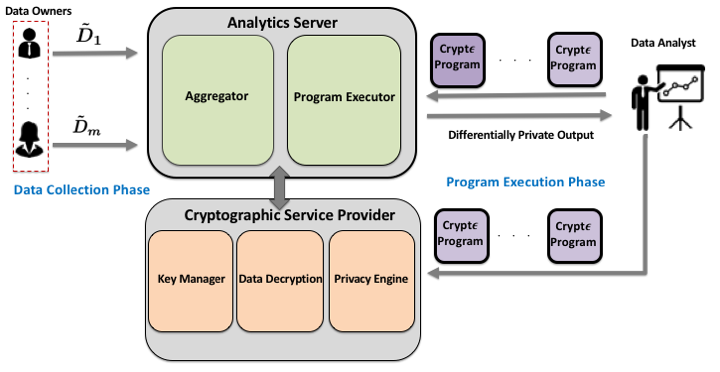
\includegraphics[height=4.1cm,width=8cm]{cryptEdiag.png}\caption{ Crypt$\epsilon$ System Setting: The  \textsf{AS} runs the Crypt$\epsilon$ programs. The \textsf{CSP} manages the cryptographic primitves. } \end{figure}

%\subsection{Notations}


This section provides an overview of \system. We begin this section with the desiderata for \system that motivates our design followed by a discourse on the different components of \system and the associated trust assumptions. Next we describe the functionality of the different modules of \system and a discussion on a few additional architectural choices we make for \system. This is followed by a brief security sketch of \system.
\subsection{Crypt$\epsilon$ Design}
The  desiderata for  the functionality of \system are as follows\\
(1) The architecture of \system should be able to support any differentially private algorithm that is permitted in the \textsf{CDP} model at the same order of accuracy guarantee as that of \textsf{CDP}, i.e. constant $O(\frac{1}{\epsilon})$ error bound.\\
(2) Raw data records cannot be stored in the clear in any server, i.e., the server(s) in \system are untrusted. \\
(3) Data owners must be  off-line.\\
Recall from our discussion in section 1, \textsf{CDP} gives constant error bounds, however it relies on a trusted server for this. In contrast \textsf{LDP} requires no trusted server but results in limited accuracy.  The first two principles thus capture \system's objective of achieving the "best of both worlds", i.e., the accuracy guarantees and expressibility of the \textsf{CDP} model with the trust assumptions similar to that of the \textsf{LDP} model. The third principle stems from the fact that another undesirable trait of \textsf{LDP} is its inherent requirement for the data owners to be on-line during every query processing.  It is so because  in \textsf{LDP} %the private data of the individuals are not collated at a single place and hence%
depending on the query at hand, every time the data owners need to compute a different noisy measurement that best answers it. This is in general a poor practice as maintaining active communication channels for the data owners might be unwieldy especially with a large number of data owners in geographically dispersed locations. \par The first desideratum can be achieved if we collate the data into a single dataset such that any measurement can be performed on the entire dataset at once followed by a single instance of noise addition as opposed to aggregation over noisy measurements on individual data. The second desideratum mandates that the data hence collected should be suitably protected via cryptographic primitives (e.g. encryption scheme). Thus the first two requirements combined, necessitates \system to be able to perform differentially private computations on the encrypted data itself. This leads us to use linear homomorphic encryption and secure computation (specifically Yao's garbled circuits)  as the cryptographic primitives of our choice for \system. Hence by virtue of secure computation, we can potentially implement all the functionalities of the \textsf{CDP} model in \system. However, bearing the practical efficiency of the cryptographic primitives in mind, we impose certain limitations on the expressibility of \system as discussed in section 3.5.  From the third desideratum, since the data owners are no longer in the loop to monitor every query answering, there is a need for a third party agent that would watchdog the overall privacy budget expenditure. 
Guided by the above principles we design a two-server model for \system with the following components
\\(1)\textbf{ Data-Owners (\textsf{DO})}-  Each data-owner $\textsf{DO}_i, i \in [m]$ has  a
private data record $D_i$ and is willing to share it only if encrypted.   \\(2)\textbf{ Analytics Server (\textsf{AS})} - The \textsf{AS} wants to run a set of differentially private programs on the dataset $\mathcal{D}=\bigcup_{i=1}^m D_i$  but has 
access only to the encrypted copies of $D_i, i \in [m]$.
\\(3)\textbf{ Cryptographic Service Provider (\textsf{CSP})} -
 The \textsf{CSP} manages the cryptographic primitives used in Crypt$\epsilon$ and interacts with the \textsf{AS} to compute the
noisy answers. It is also responsible for monitoring the privacy overall budget expenditure.
%\xh{Rather than providing all the encryption details, can we just simply have an algorithm box to summarize the interactions between these three components. Then describe the interactions and highlight the key functionalities of each component, and then the trust model. }
\subsection{Trust Model}
Both the servers, \textsf{AS} and \textsf{CSP} are completely untrusted in Crypt$\epsilon$. 
Thus from the data owners perspective the trust assumption is similar to that of \textsf{LDP}; the data owners need not place their trust in any external entity. 
However there are two modest differences in the Crypt$\epsilon$ setting from that of \textsf{LDP}.\\
 (1) We assume that the \textsf{AS} and the \textsf{CSP} do not collude with each other and follow the honest-but-curious (or semi-honest) adversary model. %That is, they always follow the instructions of the protocol faithfully but strive to learn extra information about the private records from the messages received during the execution of the protocol. 
 Moreover we assume that each data owner has a private channel with the \textsf{AS}. This is to prevent any third party (including the \textsf{CSP}) from eavesdropping. \\
 (2) The adversary (specifically the two servers \textsf{AS} and  \textsf{CSP}) is now reduced to a computationally bounded one as opposed to the information theoretic unbounded adversary  in \textsf{LDP}.
\subsection{Crypt$\epsilon$ Modules}

\stitle{Cryptographic Service Provider (\textsf{CSP})}\\
(1)\textbf{ Cryptographic Key Manager }- The foremost duty of the \textsf{CSP} is to initialize the encryption scheme of Crypt$\epsilon$. This task is handled by the \textit{Cryptographic Key Manager} module which generates the key pair $(sk,pk)$ for the \textsf{labHE} scheme. It stores the secret key, $sk$ with itself and releases the public key, $pk$. Note that since only the \textsf{CSP} has access to the secret key $sk$, it is the only entity capable of decryption in Crypt$\epsilon$.\\
(2)\textbf{ Data Decryption }- The \textsf{CSP} being the only entity capable of decryption,  any measurement of the data (even noisy) has to involve the \textsf{CSP}. The \textit{Data Decryption} module is tasked with handling all such interactions with the \textsf{AS}. \\
(3)\textbf{ Privacy Engine }- Crypt$\epsilon$ starts of with a total privacy budget of $\epsilon^B$ which is unanimously agreed upon by all the data owners. Note that the mechanism of deciding $\epsilon^*$ should be piloted by social prerogatives \cite{e1,e2} 
and is currently outside the scope of Crypt$\epsilon$. For executing every program, the \textsf{AS} has to interact with the \textsf{CSP} at least once (for decrypting the noisy answer) thereby giving the \textsf{CSP} the opportunity to monitor the \textsf{AS}'s actions in terms of privacy budget expenditure. The \textit{Privacy Engine} module hence maintains a public ledger that records the privacy budget spent in executing every individual program. Once the privacy cost incurred reaches the capped limit of $\epsilon^B$, the \textsf{CSP} refuses to decrypt any further answers thereby ensuring that the privacy budget is not exceeded.  The ledger is completely public allowing any data owner to verify it as and when desired.\\\\
\stitle{Data Owners (\textsf{DO})}\\
(1)\textbf{ Data Encoder} -  Each data owner $\textsf{DO}_i, i \in [m]$ has a private data record $D_i$ of the form $\langle A_1,...A_l\rangle$ where ${A}_j$ is an attribute. At the very outset, every data owner  $\textsf{DO}_i$ represents his/her private record $D_i$ in its respective per attribute one-hot-coding format. The one-hot-coding is a way of representation for categorical attributes and is illustrated by the following example. 
If the database schema in \system is given by  $\langle Age,Gender\rangle$ then corresponding one-hot-coding representation for a data owner $DO_i, i \in [m]$ with the record $\langle 30, Male\rangle$, is given by $\tilde{D_i}=\langle[\underbrace{0,\ldots,0}_{29},1,\underbrace{0,\ldots,0}_{70}],[1,0]\rangle$. \\
(2)\textbf{ Data Encryption} - The \textit{Data Encryption} module stores the public key $pk$ of the labHE scheme used in Crypt$\epsilon$ which is announced by the CSP. This key is used for an element-wise encryption of the data owners encoded record of per attribute one-hot-codings. In our aforementioned example, we get $\mathbf{\tilde{D}}=\langle[\underbrace{labEnc_{pk}(0),\ldots}_{29},labEnc_{pk}(1),\\\underbrace{\ldots,labEnc_{pk}(0)}_{70}],
[labEnc_{pk}(1),labEnc_{pk}(0)]\rangle$. Finally the data owner sends this encrypted record to the \textsf{AS} via a secure channel.This is the only interaction that a data owner ever participates in, all the program executions are carried out by the \textsf{AS} and the \textsf{CSP} with the data owners being completely off line.\\\\
\stitle{Analytics Server (\textsf{AS)}}\\
(1)\textbf{  Aggregator} - The \textit{Aggregator} collects the encrypted records $\mathbf{\tilde{D_i}}$ from each of the data owners $\textsf{DO}_i$ and collates them into a single encrypted database $\boldsymbol{\tilde{\mathcal{D}}}$. %Note that in contrast, the server in the \textsf{CDP} model, being trusted, stores the data in the clear whereas in the \textsf{LDP} model the untrusted server stores appropriately randomized (noisy) data.   
\\(2)\textbf{ Program Executor }- The \textit{Program Executor} is the most important module of the \textsf{AS} and is tasked with the execution of Crypt$\epsilon$ programs. It takes as input a Crypt$\epsilon$ program from an external analyst, alongside the appropriate privacy parameter $\epsilon$ and releases the differentially private output computed with the assistance of the \textsf{CSP}. Crypt$\epsilon$ supports 9 different primitives on the encrypted data and a Crypt$\epsilon$ program is an execution plan expressed as a sequence of these Crypt$\epsilon$ primitives. The primitives can be broadly classified into two types- transformation primitives and measurement primitives. Transformation primitives allow certain modifications on the encrypted data and are performed almost entirely by the \textsf{AS}. The measurement primitives on the other hand reveal some noisy measurement on the data and requires interaction with the \textsf{CSP}. A typical Crypt$\epsilon$ program execution consists of  a series of transformation on the encrypted data followed by a measurement primitive involving the \textsf{CSP} to decrypt the noisy answer. Both the \textsf{AS} and the \textsf{CSP} partake in the computation of the random noise to be added to the program output. This two-fold noise addition is necessary because  had only one of them added the noise, then after the release of the differentially private output, that party can simply subtract out the noise to reveal the true private answer. Since in Crypt$\epsilon$ the point of noise addition is just at the two servers, unlike at every individual in \textsf{LDP}, we are able to get constant error bounds just like in \textsf{CDP} (see section 7.1). 
\subsection{Crypt$\epsilon$ at work}
The complete workflow of Crypt$\epsilon$ is outlined as follows\\(1) \textbf{ Setup Phase} - This is the very first step in Crypt$\epsilon$ where the key manager of \textsf{CSP} generates the key pair for labHE $(sk,pk)$, publishes $pk$ and stores $sk$. \\(2) \textbf{ Data Collection Phase }- In the next phase, the $\textit{Data 
Encoder}$ and $\textit{Data Encryption}$ modules of every data owner, work to produce the encrypted data records which are then submitted to the \textsf{AS}. The data owners are relieved of all other duties in the Crypt$\epsilon$ setting and can go completely off-line. The $\textit{Aggregator}$ module of the \textsf{AS} then aggregates these encrypted records into a single encrypted database $\boldsymbol{\tilde{\mathcal{D}}}$. \\(3) \textbf{ Program Execution Phase} - In this phase, the \textsf{AS} executes a Crypt$\epsilon$ program with some interaction with the \textsf{CSP}  and generates a differentially private output.  \\
The \emph{Setup} and \emph{Data Collection} phases occur just once at the very beginning, every subsequent program  is handled via the corresponding  \emph{Program Execution} phase. Figure 1 shows the diagrammatic representation of \system. A comparative analysis of \system, \textsf{CDP} and \textsf{LDP} is presented in Appendix Table 5.

 %in between that of the central differential privacy model and the local differential privacy model - although it is definitely much weaker than that of the central differential privacy model, Crypt$\epsilon$'s trust model is slightly stronger as compared to that of the local differential privacy model owing to the aforementioned premises. 
%The formal security analysis for \system is presented in Appendix section B. 
\begin{comment}
learn any other information about the private datasets Di beyond what is revealed by the
model itself. Even in the case that one of the two servers (MLE or CSP) colludes with some
of the data-owners, they should learn no extra information about the data held by the
honest data-owners. In order to achieve this goal we design a system that can be seen as
multi-party protocol run by the m +2 parties mentioned before and specified by a sequence
of steps. This system (described in Section 4) has the following two-phase architecture:
We assume that the Evaluator and the CSP do not
collude. Each one may try to subvert the system as
discussed above, but they do so independently. More
precisely, at most one of these two parties is malicious:
this is an inherent requirement without which security
cannot be achieved.
• We assume that the setup works correctly, that is all
users obtain the correct public key from the CSP. This
can be enforced in practice with appropriate use of
Certificate Authorities.
Note that is true for any cryptographic primitive and is 
The can actually be avoided by removing the . m+1 secure computation where However this is Thus by capturing the we are having an huge efficincy gain now that teh problem is reduced to antwo-party

\subsection{Protocols} \xh{This might go first with the algorithm box or figure.}
In this section, for each of the three entities we list down the interactions that are initiated by them.
\begin{itemize}\item CSP- The foremost duty of the CSP is to initialize the encryption scheme of Crypt$\epsilon$. Specifically the CSP generates the key pair $(sk,pk)$ for the labeled homomorphic encryption. It stores $sk$ with itself and makes $pk$ public. Note that since only the CSP has access to the secret key $sk$, it is the only entity capable of decryption in Crypt$\epsilon$.
\item Data owners- Recall that each data owner owns a single private record which he/she shares with the AS in the encrypted form as follows. First every data owner represents his/her record in its respective per attribute one-hot-encoding format. For example, if the database schema is given by  $D=<Age,Gender>$ then a data owner with the record $<30, Male>$ would firstly represent it as $\mathcal{E}(D)=<[\underbrace{0,\ldots,0}_{29},1,\underbrace{0,\ldots,0}_{70}],[1,0]>$. This is followed by an element-wise encryption of this record of per attribute one-hot-encodings using the pubic key $pk$. In our aforementioned example, we get $\mathbf{D}=<[\underbrace{Enc(0),\ldots}_{29},Enc(1),\underbrace{\ldots,Enc(0)}_{70}],[Enc(1),Enc(0)]>$. Finally the data owner sends this encrypted record to the AS. Note that this is the only interaction that a data owner ever participates in. All the  query answering are carried out by the AS and the CSP with the data owners being completely off line. \item AS - After receiving the encrypted records from each of the data owners, the AS first collates them into a single encrypted database $\mathbf{\tilde{D}}$. For any subsequent query answering, $\mathbf{\tilde{D}}$ is subjected it to a series of transformations most of which are carried out by the AS by itself. However since the CSP is the only entity capable of decryption, for getting any measurement (even noisy) in the clear the AS has to interact with it. There are precisely two types of interactions between the AS and the CSP \begin{enumerate}\item Yao's Garbled Circuit \item Decryption of encrypted noisy value\end{enumerate}\end{itemize}
\end{comment}

\subsection{Discussion on Crypt$\epsilon$ architecture}\label{architecture}
%\xh{We may highlight our design goals (the three desiderata) and then point to later implementation to say how we achieve them. The current writeup below has too many details that reader cannot digest.}
In this section we discuss and justify the architectural choices we make for Crypt$\epsilon$. The Crypt$\epsilon$ setting is based on the premise that there are $m$ individual data owners, each possessing a private data record, and the \textsf{AS} is the primary entity who is interested in learning certain differentially private statistics on the collective data. The primary goal is to be able to achieve the constant error accuracy guarantees of  \textsf{CDP} without relying on a trusted server. %In principle, cryptographic secure multi-party computation should be able to handle this. However, incautious implementations of cryptographic primitives can be prohibitively costly. 
This leads to the following requirements.\\
(1) We should have an efficient implementation of the cryptographic primitives that are practical.\\
(2) The \textsf{AS} should be shouldering the major chunk of the workload for any Crypt$\epsilon$ program execution. Interactions with the \textsf{CSP} should be minimal and only related to data decryption.\\
(3) In the context of differential privacy, \emph{sensitivity} is the value by which any individual can affect the output of a function. Crypt$\epsilon$ programs should allow easy sensitivity analysis for the composition of the Crypt$\epsilon$ primitives. \\
The first two requirements, have been instrumental behind our choice of using $\textsf{LHE}$ for Crypt$\epsilon$. Firstly, $\textsf{LHE}$s have very efficient implementations in practice. Moreover the homomorphism allows certain operations (addition and multiplication when extended to \textsf{labHE}) to be performed directly on the encrypted data. This enables the \textsf{AS} to perform most of the data transformations by itself which conforms to our second requirement. Specifically for every Crypt$\epsilon$ program, the \textsf{AS} processes the whole database and transforms it into concise representations (like an encrypted scalar or a short vector) which is then decrypted with the help of the \textsf{CSP}. \par It is interesting to note that we could have had an alternative implementation for Crypt$\epsilon$ where the private database is equally shared between the two servers and they engage in a secret share based secure computation protocol for computing the differentially private answers. However, this would require both the servers to do almost equal amount of work for every program. Such an arrangement would be justified only if both the servers are equally invested in learning the differentially private statistics and is ill-suited for Crypt$\epsilon$ owing to our second requirement. Additionally, a secret-share based computation would be much more communication intensive resulting in a performance hit. Yet another alternative implementation could have been to engage the $m$ data owners and the \textsf{AS} in a $m+1$ secure computation protocol. This approach has two disadvantages. Firstly, as the number of data owners grow, the communication and computation overheads of this $m+1$ secure computation protocol would get prohibitively high. Secondly, this violates our requirement of off-line data owners. Thus by introducing a separate entity in the form of the \textsf{CSP}, we factor out the onus of participating in a secure multi party computation from the data owners and capture their computation power in a secure protocol between just the \textsf{CSP} and the \textsf{AS} instead %. Note that with the \textsf{CSP} in the picture, the secure computation is now reduced to a two-party case
irrespective of the number of data owners. %Not only does this improve the efficiency of our protocols drastically but is also advantageous from the perspective of ease of system implementation and maintenance. It is so because otherwise we would have had to maintain secure channels between all pairs of data owners, which would become extremely cumbersome with large values of $m$. Moreover all the data owners would have to be online for every program execution. Hence the choice of having a separate server in the form of the \textsf{CSP} is made from the efficiency point of view.
%The second assumption of an computationally bounded adversary is inherent in semantically secure cryptographic protocols. %Another design choice for Crypt$\epsilon$ could have been to keep the data owners in the loop for every program execution such that some of the data transformations could be pushed down to them. Since the data owners can perform the transformations on the plain text and in parallel, this could potentially improve performance. However this would require the data owners to be on-line during the program execution which might be unwieldy in practice especially with a large number of geographically dispersed data owners. 
\par %Keeping the efficiency of our implementation in mind, we used only two instances of simple two-party Yao's garbled circuits for Crypt$\epsilon$. In addition, we propose two optimizations that leverage on the fact that the \textsf{AS} is satisfied with differentially private outputs; this allows  us to expend some of the privacy budget in differentially private pre-processing of the encrypted data. 
The class of programs supported by Crypt$\epsilon$ is any program that can be expressed as a composition of  Crypt$\epsilon$ primitives followed by arbitrary post-processing. Crypt$\epsilon$ supports 7 transformation primitives and 2 measurement primitives. The noisy measurements allowed are the Laplace mechanism and the Noisy max (see section 4.2), two of the most popular and standard differentially private algorithms. The main constraint behind the design of the transformation primitives is that their composition should allow seamless sensitivity analysis.  Sensitivity analysis of arbitrary relational algebraic queries is a hard problem, for e.g. sensitivity of conjunctive counting queries with join operator is unbounded \cite{sensitivity}. Hence all the transformations that Crypt$\epsilon$ supports have bounded stability \cite{PINQ} such that the sensitivity analysis of any program written using them is straightforward. In fact, we showcase that the proposed Crypt$\epsilon$ primitives are indeed very powerful, enabling us to answer practically useful queries, such as linear counting queries etc. 
\\ Recall from our discussion in section 3.1, the architecture of \system imposes no fundamental restriction on its expressibility and in theory we can enjoy the same algorithmic power as that of \textsf{CDP}. However, from the discussion above, we restrict the expressibility in the current implementation of \system to ensure practical efficiency of \system programs. Nevertheless, there is a separation between \system and \textsf{LDP} as explained in Appendix E2. via \system's feasibility for an example set of three problems namely DNF queries, variable selection problem (Noisy-Max) and computing the number of distinct values for an attribute with a very large domain.
\subsection{Crypt$\epsilon$ Security Sketch}
Here we present a brief security sketch of  Crypt$\epsilon$.  There are two security requirements for \system - \\
(1) Firstly, all the programs executed by \system  should produce differentially private outputs. \\
(2) Secondly, the views of the two servers \textsf{AS} and {CSP} should be indistinguishable from that of a true \textsf{CDP} execution (modulo our assumption of a computationally bounded adversary). In other words the transcription of all the messages exchanged between the two servers can be simulated from just the differentialy private program outputs. 
\\  For the first security requirement, recall that any measurement of the data in the clear can be performed only by the measurement primitives with at least one interaction with the \textsf{CSP}. As mentioned in the preceding section, the measurement primitives supported by \system implement the standard differentially private algorithms namely the Laplace mechanism and the Noisy-Max. Thus all \system outputs are noisy.

The formal proof of the second security requirement is presented in the  Appendix B; in this section we give the readers an intuitive understanding of why \system is secure.  From the \textsf{AS}'s perspective, it has to interact with \textsf{CSP} for any measurement of the data. Recall that in \system  both the \textsf{AS} and the \textsf{CSP} are
responsible for the noise addition. Hence, the \textsf{CSP} always adds
noise of its own before releasing the decrypted data back to the
\textsf{AS}.  Moreover, in addition to the \textit{Program Executor} module of the \textsf{AS}, the data analyst communicates the Crypt$\epsilon$ program and the privacy parameter $\epsilon$ to the \textit{Privacy Engine} module of the \textsf{CSP}. This enables the \textsf{CSP} to compute the sensitivity  of the program for itself (required while adding its own noise) thereby thwarting any privacy budget over expenditure attempts under the semi-honest assumption. As for the \textsf{CSP}, its interactions with the \textsf{AS} can be categorized as   \\$\bullet$ Yao's garbled circuits with differentially private outputs \\$\bullet $ decryption of ciphers for differentially private results \\$\bullet$ decryption of ciphers for masked data  \\ The garbled circuits are inherently semantically secure and the random masks in the third type of interactions hides the true plaintext  from the \textsf{CSP}. Thus even the \textsf{CSP} is just allowed only a differentially private view of the database.





\eat{\begin{table}[h!]
\small
\centering
\caption {Comparative analysis of the different DP models}
 \begin{tabular}{l| c c c}  \toprule
\multicolumn{1}{c}{\textbf{Features}} & \textbf{LDP}  & \textbf{CDP}  & \textbf{Crypt$\epsilon$}  \\ [0.5ex] 
 \midrule \midrule \# Servers & 1& 1 & 2\\\hline
Trust  & & & Untrusted \\  Assumption & Untrusted & Trusted & Semi Honest \\for Server &  &   &  Non-Colluding  \\ \hline
Data Storage & \multirow{2}{*}{Noisy} & \multirow{2}{*}{Clear} & \multirow{2}{*}{Encrypted} \\in Server & &  &  \\\hline
Adversary & Unbounded & Unbounded & Bounded \\\hline
 Error & $O\Big(\frac{\sqrt(n)}{\epsilon}\Big)$& $O\Big(\frac{1}{\epsilon}\Big)$ & $O\Big(\frac{1}{\epsilon}\Big)$\\\hline
 Impossibility & Everything && \\results & beyond SQ model & None & None\footnotemark\\
  [1ex] 
 \bottomrule
 \end{tabular}
\end{table}
\footnotetext{Theoretically no restriction, however practical constraints maybe present}}

%\arc{ Can add another column for Mixnets maybe?}
